\subsection{五边形模组漏电流测试}

从2021年初开始,在山大制作完成的五边形模组被陆续寄到BNL,等待测试和组装。因为这一批模组是最后组装成为前向窄隙室径迹探测器的模组,所以说需要进行长时间的高压打火测试,来保证探测器可以长时间稳定地运行。所有的探测器在山大制作完成之后均进行过长时间的打火测试,结果被记录在了每个探测器的travller当中。图\ref{fig:S18_traveller}为S18在山大进行漏电流测试时的结果。可以看到在山大测试时漏电流很稳定且低于50nA。当探测器运到BNL后,如果一个模组没有因为在运输途中遇到意外而损坏的话,在通气24小时进行干燥之后就开始进行漏电流测试。
\begin{figure}[htb]
    \begin{center}
    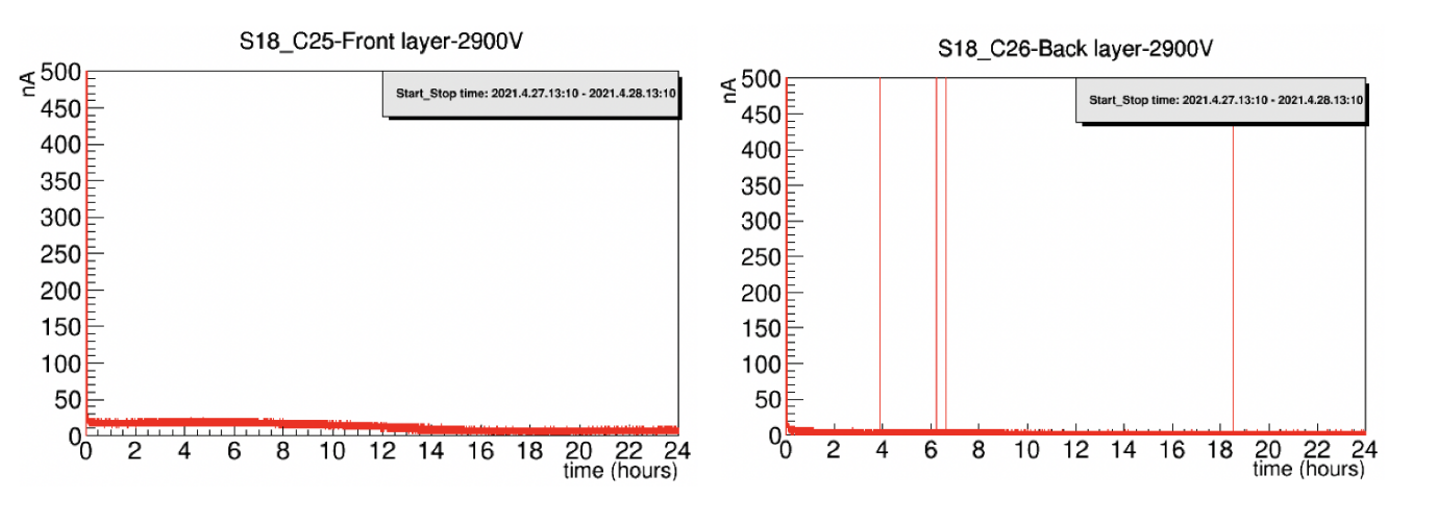
\includegraphics[width=0.8\textwidth,clip]{figures/Chapter3/S18_traveller.png}
    \end{center}
    \caption[五边形模组S18山大漏电流测试结果]{五边形模组S18山大漏电流测试结果}
    \label{fig:S18_traveller}
\end{figure}

第一批被安全寄到BNL的模组为S18和S21,首先使用了LeCory作为电源对其进行了漏电流测试,在Jarda的帮助下通过Python脚本实现了对电流数据的记录。但因为LeCory电源本身读出系统的限制,数据记录系统的记录频率仅为4.6Hz。且无法设置trip time,只能使用LeCory自己内部的设置。同时在测试环境上,相比于山大位于超净室当中测试,可以控制整个环境的湿度和温度。BNL的超净室因为被占用,所以只能在Wide Angle Hall当中进行测试,无法控制环境的温度和湿度。测试时间处于夏季,湿度为大约55\%,对整个探测器的漏电流表现还是有一定的影响。从图\ref{fig:LeakCurrent_LeCory}中可以观察到,在加上高压之后漏电流需要一段时间以后才能稳定在较低的数值。

为了保证电源和探测器的安全,整个测试过程当中电压从1000V开始当漏电流稳定以后再升高500V,当漏电流再次稳定之后再升高电压。直到升高到2900V为止。以S18-C55为例,在1000-2500V下的漏电流表现如图\ref{fig:LeakCurrent_LeCory}所示,可以看到在加高压足够的时间之后,整个探测器的漏电流都会趋于稳定,但是普遍高于山大的漏电流测试结果。当使用LeCory尝试升高电压至2900V的时候,同时进行测试的S18和S21的四个室均发生了trip。之后决定在2800V进行更长时间的Burning之后在升到2900V进行测试。但是在这个过程中发生了LeCory电源的死机,死机重启后电源的表现变得比较奇怪。决定更换电源后重新进行测试。
\begin{figure}[htb]
    \begin{center}
    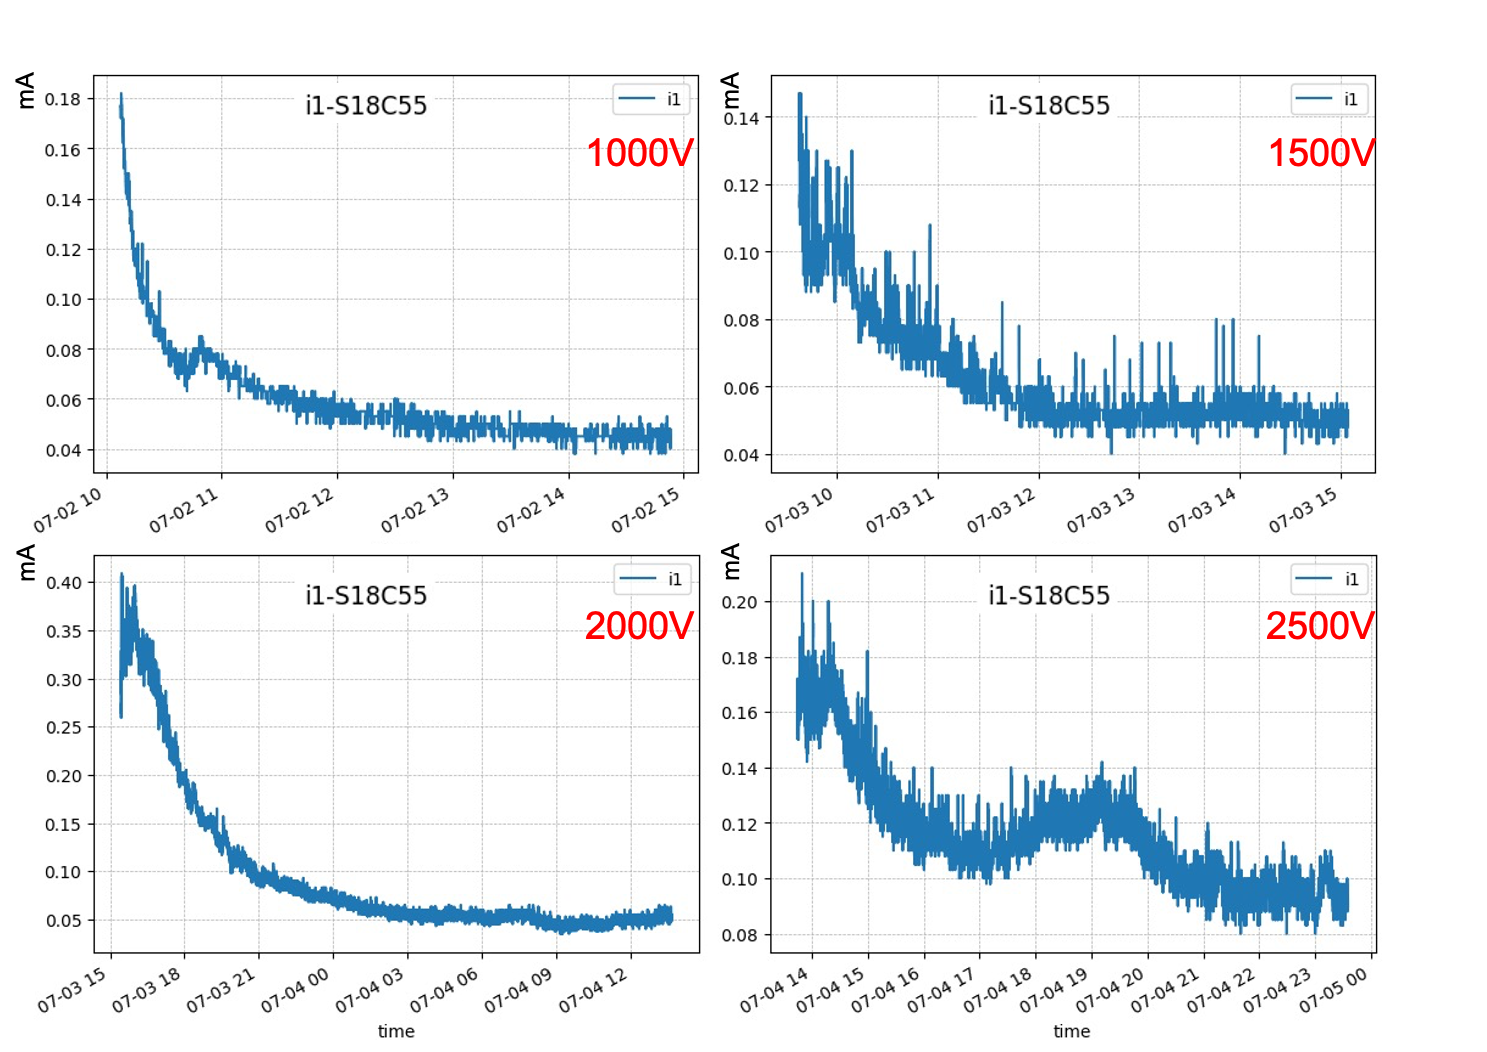
\includegraphics[width=0.8\textwidth,clip]{figures/Chapter3/LeakCurrent_LeCory.png}
    \end{center}
    \caption[五边形模组S18 BNL使用LeCory电源漏电流测试结果]{五边形模组S18 BNL使用LeCory电源漏电流测试结果}
    \label{fig:LeakCurrent_LeCory}
\end{figure}

之后的测试当中电源被更换为CANE SY5527,即当前向窄隙室探测器安装到STAR上之后会使用的电源。但同样因为读出系统的问题,电流数据记录的频率仅为约1.4Hz。但相比于LeCory电源,SY5527可以设置trip time。使用SY5527时的测试设置如表\ref{tab:SY5527Settting}所示。更换成SY5527之后测试方法和用LeCory测试时一样,从500V开始电压逐步升高,当漏电流稳定之后再将电压升到更高的电压。以S16-C22为例,在500、1000、1500、2500V时的电压表现分别如图\ref{fig:LeakCurrent_SY5527}所示。相比于LeCory,在低电压时SY5527的漏电流整体要高于LeCory的漏电流,约为200-300nA,但更加的稳定。在低电压下漏电流表现很稳定之后开始将电压升到2900V进行测试。
\begin{table}[h!]
    \centering
    \caption{SY5527漏电流测试设置}
    \label{tab:SY5527Settting}
    \begin{tabularx}{1\textwidth} {| >{\centering\arraybackslash}X |>{\centering\arraybackslash}X |>{\centering\arraybackslash}X |>{\centering\arraybackslash}X |}
        \hline
        trip current & trip time & ramp up speed & ramp down speed \\
        \hline
        2 ${\rm \mu A}$& 0.1s & 10 V/s & 20 V/s \\
        \hline
    \end{tabularx}
\end{table}
\begin{figure}[htb]
    \begin{center}
    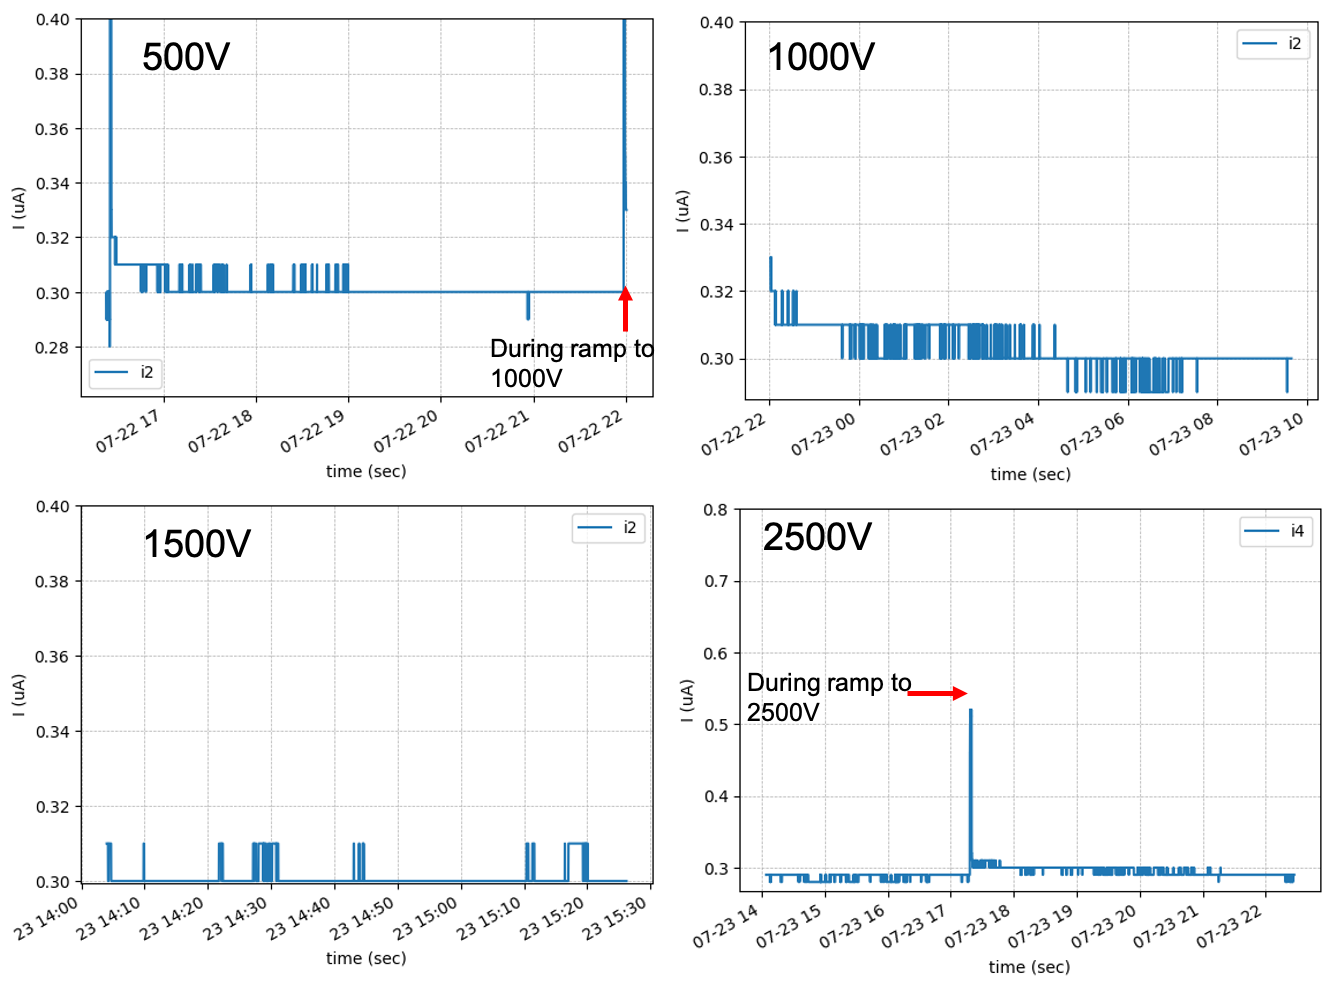
\includegraphics[width=0.8\textwidth,clip]{figures/Chapter3/SY5227LeakCurret.png}
    \end{center}
    \caption[五边形模组S16 BNL使用CANE SY5527电源漏电流测试结果]{五边形模组S16 BNL使用CANE SY5527电源漏电流测试结果}
    \label{fig:LeakCurrent_SY5527}
\end{figure}

当电压升到2900V,漏电流的表现依旧相对稳定,约为500nA。但是观察到了比较奇怪且尖锐的峰,如图\ref{fig:LeakCurrent_SY5527_2900}所示。在8月1日的晚上出现了一个很尖锐的峰,在检查数据的时候发现峰值可以达到10${\rm \mu A}$级别,持续时间也大于所设置的tirp时间0.1s。且并不是一个漏电流逐渐上升的过程,漏电流会突然跳到很大的数值并在大约2-3s后再次回到之前的值。在之后的测试中也多次发现了这样奇怪的峰,但没有发生trip现象,探测器仍然稳定工作。最后经过排查怀疑是电源自带的电流读出系统的问题。在所有的五边形模组通过了漏电流测试以后前向窄隙室径迹探测器的组装工作随后开始。
\begin{figure}[htb]
    \begin{center}
    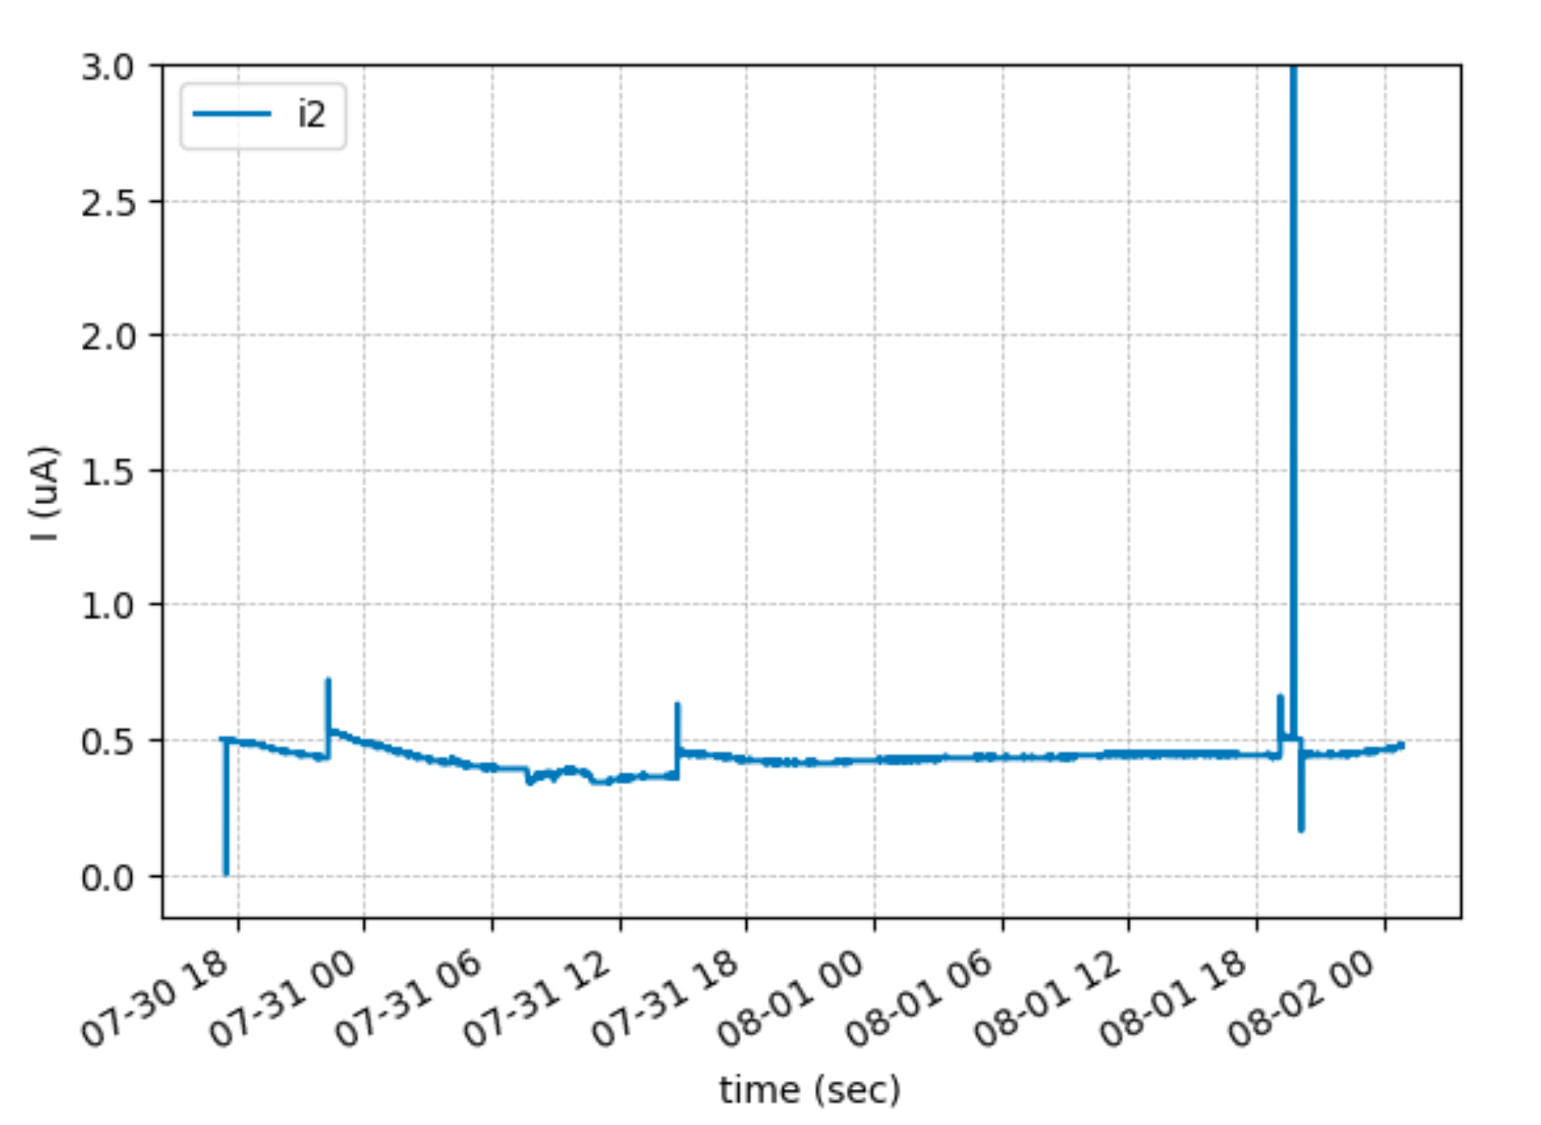
\includegraphics[width=0.8\textwidth,clip]{figures/Chapter3/LeakCurrent_SY5527_2900.png}
    \end{center}
    \caption[五边形模组S16 BNL使用CANE SY5527电源电压为2900V漏电流测试结果]{五边形模组S16 BNL使用CANE SY5527电源电压为2900V漏电流测试结果}
    \label{fig:LeakCurrent_SY5527_2900}
\end{figure}